%\documentclass[aspectratio=43]{beamer}
\documentclass[c]{beamer}
\usetheme{intridea}  %% Themenwahl

\usepackage[ngerman]{babel} 
\usepackage[T1]{fontenc}    % richtige Silbentrennung
\usepackage[utf8]{inputenc} % Umlaute etc.!
\usepackage{eurosym}
\usepackage{tikz}

\usetikzlibrary{arrows,decorations.pathmorphing,backgrounds,fit,positioning,shapes.symbols,chains}

%1

\title{Freifunk Helgoland}
\author{hamburg.freifunk.net}
\date{2014/Dez/12}

%2
\begin{document}
\maketitle

\begin{frame}{Was ist freifunk?}
	\begin{itemize}
		\item Initiative für freie, offene, kostenlose Netzwerke
		\item Öffentlich - freifunk steht jedem offen, als Nutzer oder Anbieter
		\item Im Besitz der Gemeinschaft - Wird von den Menschen betrieben, die es nutzen
		\item Nicht kommerziell
		\item Ausschliesslich freie, quelloffene Programme
		\item Netzneutral - keine Manipulation der Datenströme
		\item In  \href{http://freifunk.net/wie-mache-ich-mit/community-finden/}{139 Orten} gibt es bereits Freifunknetze mit mehr als 7500 Zugangspunkten
	\end{itemize}
\end{frame}

%3
\begin{frame}{Freifunkknoten}
	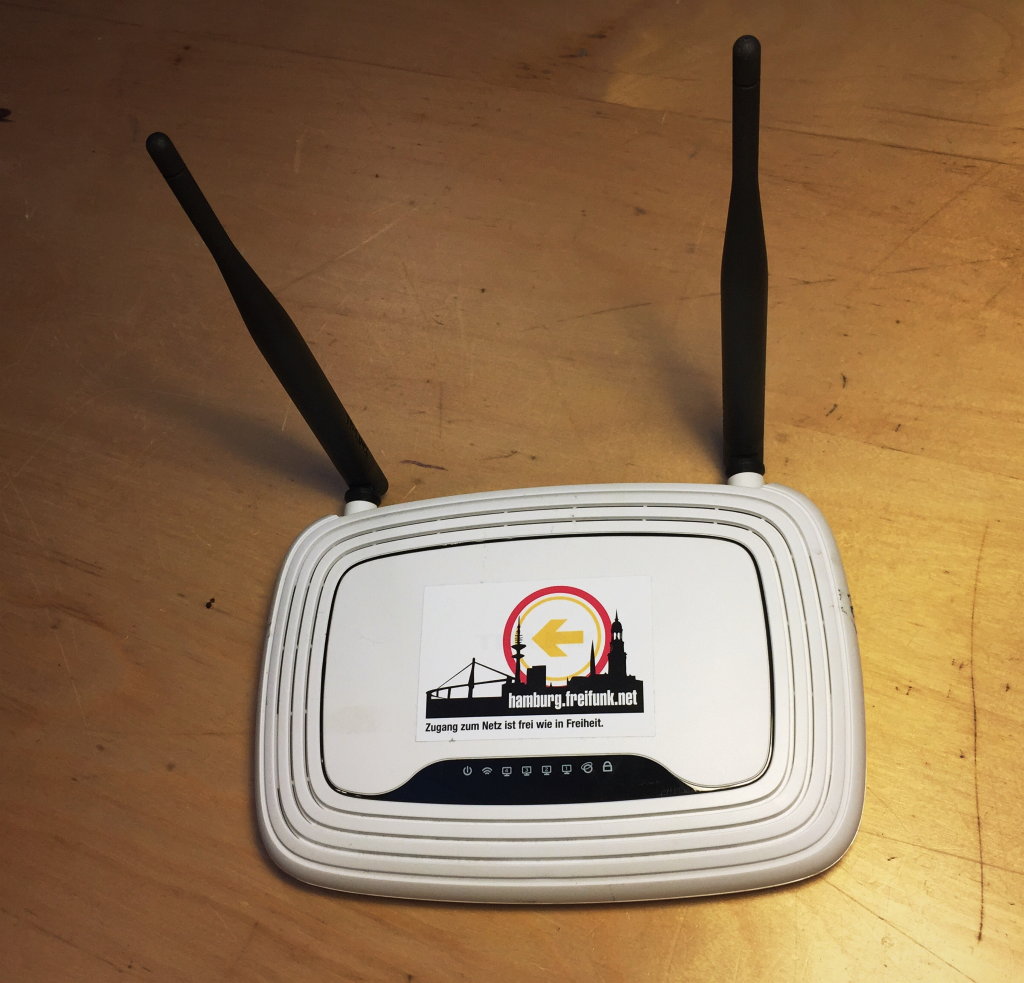
\includegraphics[width=.6\textwidth]{Bilder/841}
\end{frame}


%4
\begin{frame}{Mit freifunk ins Internet}
	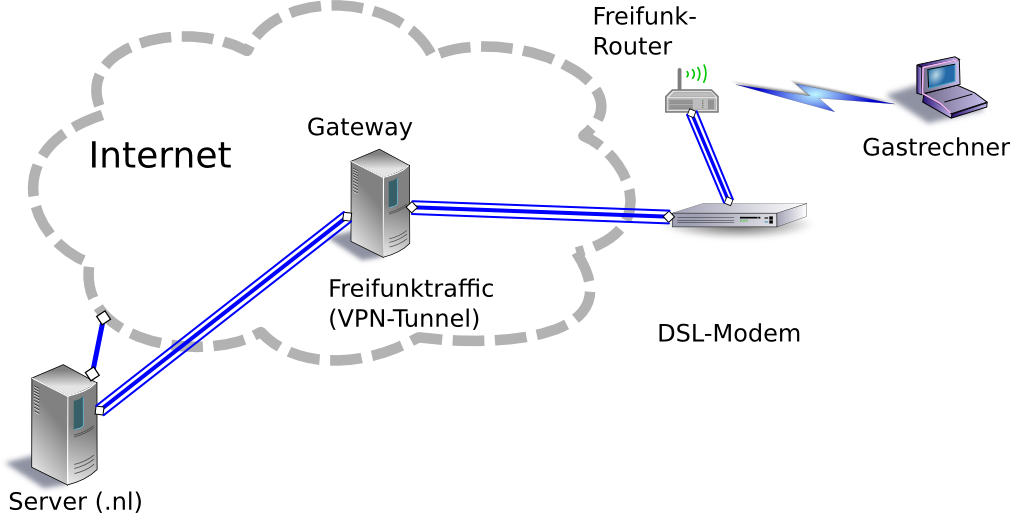
\includegraphics[width=\textwidth]{Bilder/Freifunk_Knotenanbindung}
\end{frame}


%9
\begin{frame}{Knotenkarte}
	\begin{center}
		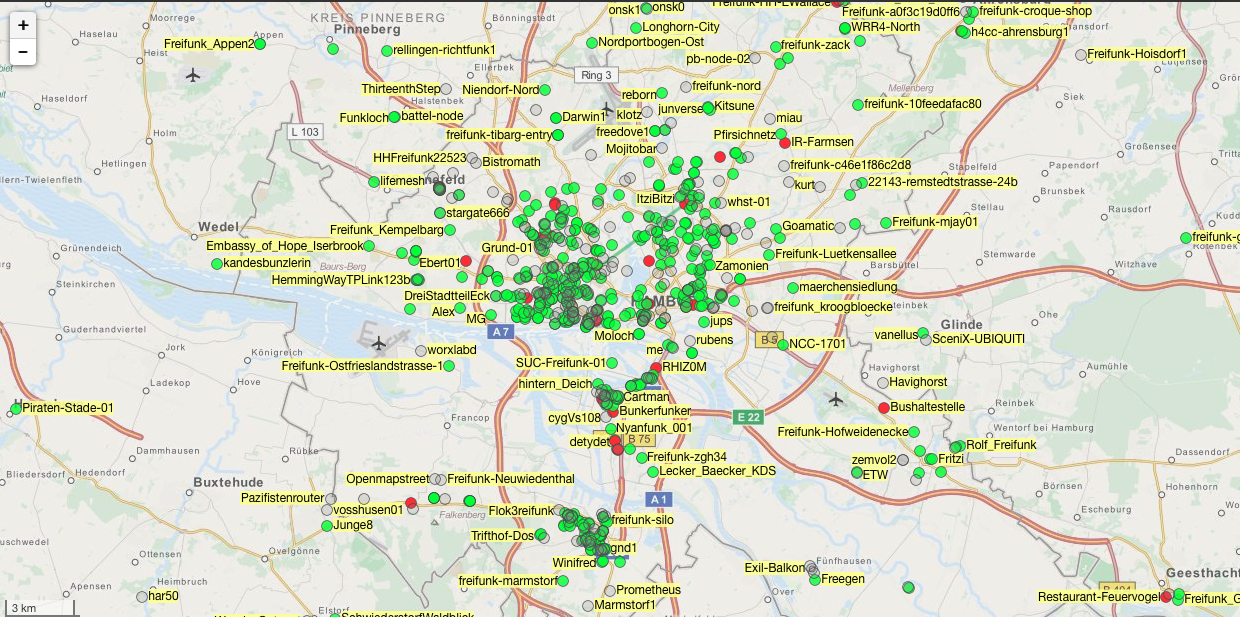
\includegraphics[width=.8\textwidth]{Bilder/knotenkarte1}
	\end{center}
\end{frame}



%10
\begin{frame}{Sicherheit}
	\begin{itemize}
		\item Da freifunk kein Kennwort nutzt, ist die Funkstrecke zum Zugangspunkt (wie bei allen offenen WLANs) unverschlüsselt
		\item Wie sonst im Netz auch, sollte nach Möglichkeit Ende-zu-Ende-Verschlüsselung genutzt werden
		\item Verbindung freifunk-Knoten zu Gateway läuft durch VPN und ist verschlüsselt --> kein Zugriff auf das Heim-/Firmennetzwerk möglich
	\end{itemize}
\end{frame}


%11
\begin{frame}{Störerhaftung}
	\begin{itemize}
		\item Die Zugangspunkte gehen nicht direkt in das Internet
		\item Es wird über das Internet eine verschlüsselte VPN-Verbindung zu den Gateways aufgebaut, die nicht der Störerhaftung unterliegen
	\end{itemize}
\end{frame}


%13
\begin{frame}{Richtfunknetz}
	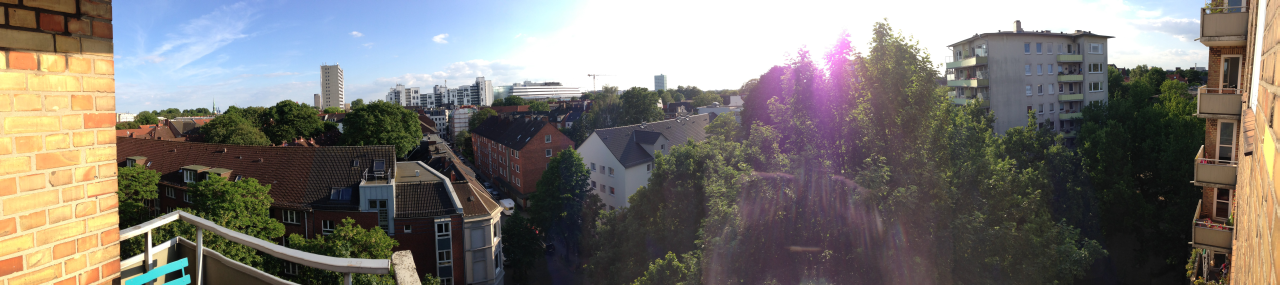
\includegraphics[width=\textwidth]{Bilder/esmarch95}
	\begin{columns}
		\begin{column}{0.7\textwidth}
			\begin{itemize}
				\item Möglichkeit das Netz durch Richtfunkstrecken von Haus zu Haus weiter zu leiten
				\item Erhöhte Standorte (z.B. Kirchturm) sind von Vorteil
			\end{itemize}
		\end{column}
		\begin{column}{0.3\textwidth}
			\begin{center}
				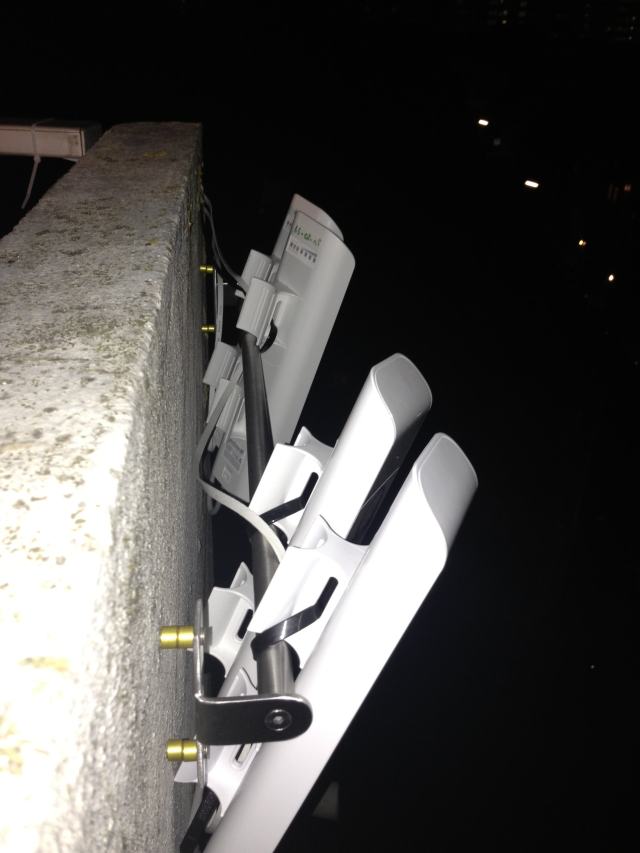
\includegraphics[width=.8\textwidth]{Bilder/esmarch95-2}
			\end{center}
		\end{column}
	\end{columns}
	
\end{frame}



%17
\begin{frame}{}
	\begin{columns}
		\begin{column}{1\textwidth}
			\begin{itemize}
				\item Netz: hamburg.freifunk.net
				\item Ansprechpartner: Alexander Bernhardt 
				\item Mail: bernhardt@hauptsache.net
		\end{itemize}
			\begin{center}
				
\includegraphics[width=0.2\textwidth]{Bilder/cc-by}
			\end{center}
		\end{column}
	\end{columns}
\end{frame}

\end{document}